\documentclass{llncs}%

\usepackage{booktabs} % For formal tables
\usepackage{todonotes}
\usepackage{amsmath,amssymb,amsmath,amsfonts}
\usepackage{xspace}
\usepackage{enumerate}
\usepackage{xcolor} 
\usepackage{tikz}   
\usepackage{pifont} 
\usepackage{bm}
\usetikzlibrary{matrix,arrows.meta,fit,decorations.markings,intersections,arrows,positioning,shapes.misc}  
\usepackage{tcolorbox} 
\tcbuselibrary{raster,skins}
\usepackage{rotating}    
\newcommand*\circled[1]{\tikz[baseline=(char.base)]{
    \node[shape=circle,draw,inner sep=0.5pt] (char) {#1};}}    
\usepackage{tikz-cd}  

%================================================

\DeclareMathAlphabet{\mathsfit}{T1}{\sfdefault}{\mddefault}{\sldefault}
\SetMathAlphabet{\mathsfit}{bold}{T1}{\sfdefault}{\bfdefault}{\sldefault}


%================================================
\def\bigcupe{\, {\bigcup\hspace{-8.8pt} \scalebox{0.7}{\ensuremath{\emptyset}}} \; \;}
\def\bigcuperun{\, {\bigcup\hspace{-7.3pt} \scalebox{0.6}{\ensuremath{\emptyset}}} \;}
\newcommand{\powerset}[1]{\ensuremath{2^{#1}}} % power set
\newcommand{\PF}{\ensuremath{\mathcal{F}_{p}}\xspace} % Abstract argumentation framework
\newcommand{\F}{\ensuremath{\mathcal{F}}\xspace} % Abstract argumentation framework
\newcommand{\args}{\ensuremath{\mathsf{A}}\xspace} % Set of arguments
\newcommand{\argsp}{\ensuremath{\mathsf{A}_p}\xspace} % Set of arguments
\newcommand{\atts}{\ensuremath{\mathsf{R}}\xspace}
\newcommand{\attsp}{\ensuremath{\mathsf{R}_p}\xspace}
\newcommand{\attacks}{\ensuremath{\rightarrow}\xspace}
\newcommand{\labelf}{\ensuremath{\mathcal{L}}\xspace}
\newcommand{\attackers}[2]{\ensuremath{\mathcal{F}_{#1}(#2)\xspace}} % Attacker set
\newcommand{\PA}{\ensuremath{P_{\argsp}}\xspace} 
\newcommand{\PD}{\ensuremath{P_{\attsp}}\xspace} 
\newcommand{\AFC}{\ensuremath{\F=(\args,\atts)}\xspace} % Definition of an abstract argumentation framework
\newcommand{\PFC}{\ensuremath{\PF=(\argsp,\attsp,\PA,\PD)}\xspace}
\newcommand{\cA}{\ensuremath{\mathcal{A}}} % some argument
\newcommand{\cB}{\ensuremath{\mathcal{B}}} % some argument
\newcommand{\cC}{\ensuremath{\mathcal{C}}} % some argument
\newcommand{\argin}{\ensuremath{\mathsf{in}}} % argument is in
\newcommand{\argout}{\ensuremath{\mathsf{out}}} % argument is out
\newcommand{\argundec}{\ensuremath{\mathsf{undec}}} % argument is undec

\newcommand{\Given}{\textbf{Given}\xspace}
\newcommand{\decide}{\textbf{decide}\xspace}
\newcommand{\Enumerate}{\textbf{enumerate}\xspace}
\newcommand{\return}{\textbf{return}\xspace}

\newcommand{\af}{AF}

\newcommand{\co}{\mathbf{co}}
\newcommand{\pr}{\mathbf{pr}}
\newcommand{\st}{\mathbf{st}}
\newcommand{\sst}{\mathbf{sst}}
\newcommand{\stg}{\mathbf{stg}}
\newcommand{\gr}{\mathbf{gr}}
\newcommand{\id}{\mathbf{id}}
\newcommand{\eg}{\mathbf{eg}}

\newcommand{\se}{\mathbf{SE}}
\newcommand{\ee}{\mathbf{EE}}
\newcommand{\dc}{\mathbf{DC}}
\newcommand{\ds}{\mathbf{DS}}

\newcommand{\quot}[1]{``#1''}

\newcommand{\ryuta}[1]{{\color{magenta}{#1}}} 
\newcommand{\francesco}[1]{{\color{purple}{#1}}}
%================================================

\begin{document}


\title{Title: Research Proposal}

\author{Ryuta Arisaka\inst{1}, Francesco Santini\inst{2}}
\institute{
	Kyoto University, Kyoto, Japan \\
	\email{ryutaarisaka@gmail.com}
\and	
	Department of Mathematics and Computer Science, University of Perugia, Italy\\
\email{francesco.santini@unipg.it}\\
}

\maketitle
 




\begin{abstract}
???
\end{abstract}



\section{Introduction}\label{sec:intro}
Suppose the case of manslaughter where a man is pleaded guilty of killing his wife. Suppose there were 
100 similar manslaughter cases of a man killing his wife in the last 5 years, in 60 of which the suspects were charged with voluntary manslaughter, 
and in 40 of which they were charged with involuntary manslaughter. Based on those past outcomes, we may model 
judge's decision-making process as Fig. \ref{fig_stat}'s right hand side of argumentation, where $\Rightarrow$ (in any orientation) indicates a support relation  
and $\rightarrow$ (in any orientation) an attack relation. 
\begin{figure}[!h]  
\begin{tikzcd}[column sep=small,row sep=small] 
	& \text{VoluntaryManslaughter}  \arrow[dd, shift left] \\
	 \text{ManKilledWife} \arrow[Rightarrow,ur, "0.6"] \arrow[dr,Rightarrow, "0.4"] \\ 
	 & \text{InvoluntaryManslaughter} \arrow[shift left,uu]
\end{tikzcd}    
\begin{tikzcd}[column sep=small,row sep=small] 
	\parbox{2.3cm}{ManKilledWife CircumstanceA} \arrow[Rightarrow,r] \arrow[dd,shift left]& \text{VoluntaryManslaughter}  \arrow[dd, shift left] \\ \\ 
	 \parbox{2.3cm}{ManKilledWife CircumstanceB} \arrow[uu,shift left] \arrow[r,Rightarrow] & \text{InvoluntaryManslaughter} \arrow[shift left,uu]
\end{tikzcd}    
	\caption{\textbf{Left}: argumentation with disjunctive branches from acceptance of ManKilledWife. \textbf{Right}: argumentation 
	with no disjunctive branches from acceptance of ManKilledWifeCircumstanceA or ManKilledWifeCircumstanceB.} 
	\label{fig_stat} 
\end{figure} 
It intends to prescribe to the current manslaughter case the following disjunctive guideline: statistically, by 60\% chance, 
it is a voluntary manslaughter, and by 40\% chance, it is an involuntary manslaughter. 

\subsection{Research problems} 
While the statistically disjunctive argumentation provides an intuitive overview of court decisions on manslaughter cases,  
it is rather evident that the judge cannot base his/her judgement on the statistics for his/her decision 
on the present manslaughter case. Between voluntary and involuntary manslaughter, 
the difference in severity of penalty is in fact too huge to tolerate probabilistic judgement. 
What the judge will need is more detail that can somehow split ManKilledWife argument into the argumentation 
on the right hand side 
of Fig. \ref{fig_stat}, so that if the current manslaughter case happens to fall into CircumstanceA, then 
the judge can deterministically conclude the case as voluntary manslaughter, and if 
it should fall into CircumstanceB, then the judge can deterministically conclude the case as involuntary manslaughter. 
Or if it does not fall into either, then the judge can, again deterministically, conclude the present case 
to be an exception to past decision-makings.  

However, how the splitting (we call the arguments as the result of splitting `splits') may be achieved is the primary issue coming with several associated criteria. 
\begin{description} 
	\item[Mutual exclusion:] Splits of an argument lead to distinct decisions. 
	\item[Completeness:] Splits of one argument taken together recover the original argument for the past cases. 
	\item[Generality:] Splits are general enough for future uses of the argumentation as a decision-making guideline. 
\end{description} 

\begin{example} 
  To illustrate each of the three criteria, let us suppose the following. The left table shows the past 100 cases and the right table 
	shows the present case. For simplicity, there were 30 past cases all falling under the first description, 
	30 past cases all under the second description, and 40 past cases all under the third description. \\\\ 
	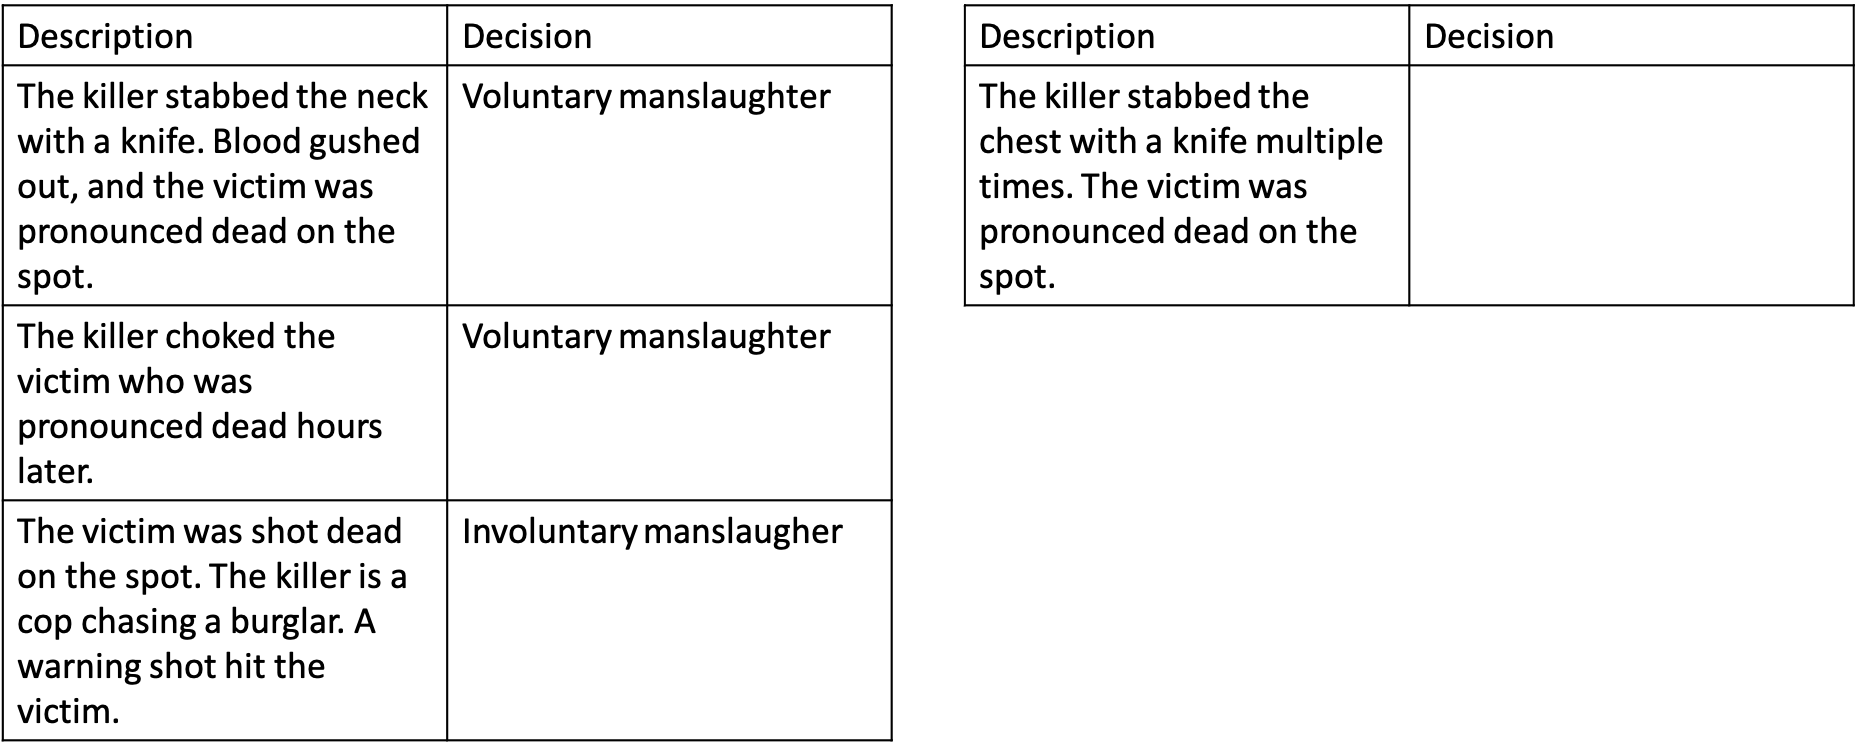
\includegraphics[scale=0.4]{table1.png}

	\begin{itemize} 
		\item Suppose CircumstanceA is ``the wife dead on the spot'' and ``the man used a knife", and CircumstanceB is ``the wife dead on the spot" 
			and ``the man used a gun".  Then, The first description fits in CircumstanceA, and the third description is under CircumstanceB. 
			Since the first description's decision is voluntary manslaughter, while the third description's decision is involuntary manslaughter, 
			we have achieved a mutually exclusive splitting. However, the second description is neither CircumstanceA nor CircumstanceB. 
			Hence they fail to satisfy the criterion of completeness.  
		\item Suppose CircumstanceA is ``XXXX'' and CircumstanceB is ``YYYY''. 
		\item Suppose CircumstanceA is ``ZZZZZ" and CircumstanceB is ``WWWWW".
	\end{itemize} 
	


\end{example} 




\section{Related Work}\label{sec:related}

\begin{itemize}
    \item Formal argumentation and ontologies (Descritpion Logic) \cite{ontology}
    \item Disjunctive frameworks
\end{itemize}



\section{Background}\label{sec:bg}



\section{Conclusions and Future Work}\label{sec:conclusion}





\pagebreak 

\section*{Research problems and objectives} 
The current shortage of argumentation research \ryuta{correct me if this is not correct....} is, 
modelling of specific argumentations that have been already conducted is studied extensively, but reusability of the derived
argumentation has been seldom shed light on. As such, while useful as a formal model to orderly understand a decision-making process,  
a new specific argumentation case has to be modelled anew, which is expensive and tedious. That is the same problem 
as model checking suffers from. 

Therefore the aims: 
\begin{enumerate} 
	\item  We develop a formal framework which enables construction of a general argumentation from similar past decisions that 
		can act as a guideline for a similar future decision-making case. 
	\item 
\end{enumerate}

\section*{Significance} 
\begin{enumerate} 
	\item We fortify XAI by having a formal mechanism to explain criteria for decision-makings. 
	\item 
\end{enumerate}
\bibliographystyle{splncs03}%splncs
\bibliography{main}
\end{document}
